\begin{scanpage}{0171}{153}
\begin{center}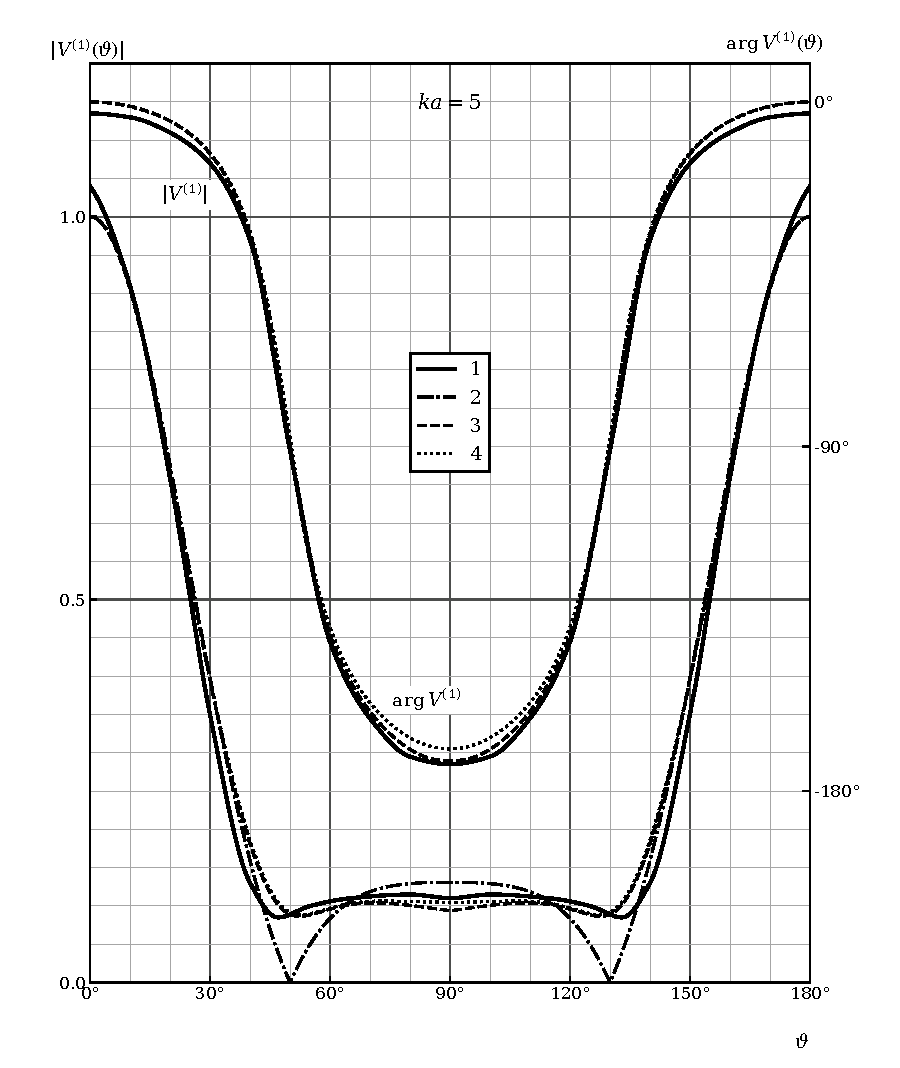
\includegraphics[width=.58\linewidth]{images/recreated/c-0171-fig67.pdf}\par
Figure 67. The function $V^{(1)}(\vartheta)$ for a disk with normal incidence of a plane wave (curve 4). Curves 1, 2 and 3 from Figure 20 are drawn for comparison.
\end{center}
depend on the secondary diffraction here are small (on the order of 1 dB) when $ka=\pi$, $kl=10\pi$, and the equations are substantially more complicated, we shall not cite them here.

In the problems investigated above, the edge waves have the character of cylindrical or spherical waves---that is, they decrease rather rapidly with the distance from the edge. Therefore, in the case when the linear dimensions of the faces are approximately two wavelengths, it is sufficient to limit ourselves to a consideration
\end{scanpage}
